\documentclass[11pt]{article}
\usepackage[margin=1in]{geometry}
\usepackage{amsmath, amssymb, amsthm}
\usepackage{tikz}
\usetikzlibrary{arrows.meta, calc, backgrounds, fit, positioning}
\usepackage{xcolor}
\usepackage{microtype}
\usepackage{hyperref}
\hypersetup{colorlinks=true, linkcolor=blue!50!black, citecolor=blue!50!black, urlcolor=blue!50!black}

%% ---- operator notation (matches the "Formalising the Merge" writeup) ----
\newcommand{\ids}{\mathsf{ids}}
\newcommand{\anc}{\mathsf{anc}}
\newcommand{\el}{\mathsf{el}}
\newcommand{\climb}{\mathsf{climb}}
\newcommand{\mrg}{\mathsf{merge}}
\newcommand{\rc}{\mathsf{rc}}
\newcommand{\doo}{\mathsf{do}}
\newcommand{\resolve}{\mathsf{resolve}}
\newcommand{\Ins}{\mathsf{Ins}}
\newcommand{\Del}{\mathsf{Del}}
\newcommand{\Either}{\mathsf{Either}}
\newcommand{\contains}{\mathsf{contains}}
\newcommand{\lca}{L}

%% ---- tikz styles ----
\tikzset{
  vtx/.style     ={draw, circle, minimum size=8.5mm, inner sep=0pt, fill=blue!8,  line width=0.6pt},
  rootvtx/.style ={draw, circle, minimum size=8.5mm, inner sep=0pt, fill=black!12, line width=0.6pt, font=\bfseries},
  dead/.style    ={draw, circle, minimum size=8.5mm, inner sep=0pt, densely dashed, fill=black!4, text=black!40, line width=0.6pt},
  newv/.style    ={draw, circle, minimum size=8.5mm, inner sep=0pt, fill=green!14, line width=0.7pt},
  anc/.style     ={-{Stealth[length=2.2mm]}, line width=0.8pt},                          % node -> its anchor
  climb/.style   ={-{Stealth[length=2.2mm]}, line width=1.0pt, red!75!black, densely dashed}, % climb / rehome
  ghost/.style   ={-{Stealth[length=2mm]}, line width=0.7pt, black!28, densely dotted},
  elbl/.style    ={font=\scriptsize, text=black!60},
  capt/.style    ={font=\small\itshape, text=black!75},
}

\title{\bfseries Why the Path Matters\\[2pt]
\large A visual account of the tombstone-free, path-carrying RGA}
\author{Sal / FP Launchpad}
\date{}

\begin{document}
\maketitle
\sloppy

\begin{abstract}
\noindent
The replicated growable array (RGA) in \texttt{RGA\_Tombstone\_Free} stores only
\emph{live} elements: a delete physically removes its target, leaving no
tombstone. To stay convergent without tombstones, each operation carries the
\emph{ancestor path} of the node it references. This note explains, with pictures,
two things: \textbf{(i) why the implementation converges} --- the three-way merge
recovers a concurrently-deleted node's parent from the lowest common ancestor
(LCA); and \textbf{(ii) why the path is necessary \emph{for the single-replica
commutation proof}} --- to discharge the framework's $\doo$-commutation VC, where
there is no LCA, an insert whose anchor was deleted has nowhere to recover its
position \emph{unless it carries that position itself}. The qualification matters:
the merge alone already converges the concurrent case \emph{without} any path
(\texttt{merge\_converges\_concurrent}); it is this commutation \emph{obligation},
not operational convergence, that the path serves. We give the
counterexample that diverges without the path, the fix that the path provides, and
the asymmetry that makes the path mandatory for $\Ins$ but optional for $\Del$.
Every claim here is mechanised in Lean (\S\ref{sec:mech}).
\end{abstract}

\section{The data type: a forest of live records}

The state is a finite map $\sigma : \mathrm{id} \mapsto (\el, \anc)$ from an
identity to its element and its \emph{immediate anchor} --- the identity it was
inserted after. Identity $0$ is the root sentinel and is never stored. So a state
\emph{is} a forest rooted at $0$: an edge from a node to its anchor (Figure
\ref{fig:state}). We write $\ids(\sigma)$ for the stored identities,
$\el(\sigma,t)$ and $\anc(\sigma,t)$ for the element and anchor of $t$, and
$\contains(\sigma,t)$ for ``$t$ is live''. Records use the reference notation
$(\mathrm{id},\ \mathrm{element},\ \mathrm{anchor})$.

\begin{figure}[h]
\centering
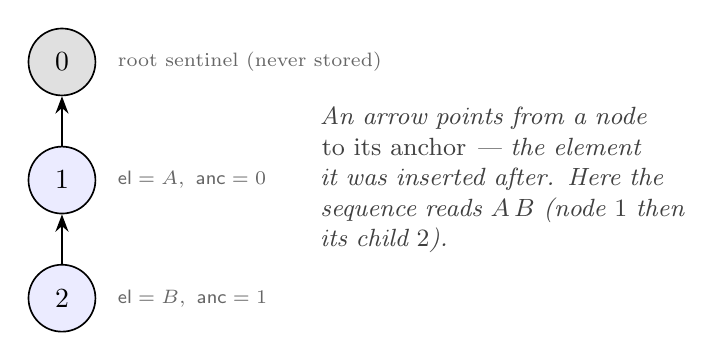
\begin{tikzpicture}
  \node[rootvtx] (r) at (0,0)    {$0$};
  \node[vtx]     (1) at (0,-1.5) {$1$};
  \node[vtx]     (2) at (0,-3.0) {$2$};
  \draw[anc] (1) -- (r);
  \draw[anc] (2) -- (1);
  \node[elbl, right=1.5mm of r] {root sentinel (never stored)};
  \node[elbl, right=1.5mm of 1] {$\el=A,\ \anc=0$};
  \node[elbl, right=1.5mm of 2] {$\el=B,\ \anc=1$};
  \node[capt, text width=4.6cm, align=left] at (5.6,-1.5)
    {An arrow points from a node \emph{to its anchor} --- the element it was
     inserted after. Here the sequence reads $A\,B$ (node $1$ then its child
     $2$).};
\end{tikzpicture}
\caption{The state as a forest. $\sigma=\{(1,A,0),(2,B,1)\}$.}
\label{fig:state}
\end{figure}

\paragraph{Operations.} There are two, and (crucially) each carries a \emph{path}
$p$ --- the ancestor chain of its referenced node, nearest first:
\begin{itemize}
  \item $\Ins(e, p, a)$ at a fresh id $t$: insert $e$ anchored at $a$. It stores
        $(t, e, \resolve(\sigma, a\!::\!p))$, where $\resolve$ returns the first
        \emph{live} candidate in its list, else $0$. When $a$ is live this is just
        $a$; when $a$ is dead it climbs $p$ to the nearest live ancestor.
  \item $\Del(p, x)$: \emph{splice} out $x$ --- physically remove it and re-parent
        its children to $\resolve(\sigma, p)$, the nearest live ancestor of $x$.
        No tombstone is kept.
\end{itemize}

Figure \ref{fig:splice} shows the defining move of a tombstone-free delete: the
splice. Deleting $2$ removes it and lifts its child $3$ one level, onto $2$'s
parent $1$.

\begin{figure}[h]
\centering
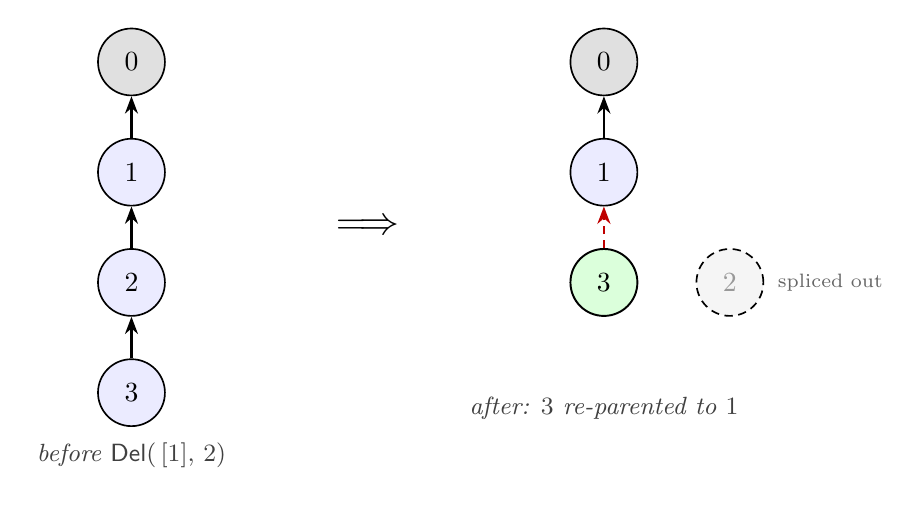
\begin{tikzpicture}
  % before
  \node[rootvtx] (r) at (0,0)    {$0$};
  \node[vtx]     (1) at (0,-1.4) {$1$};
  \node[vtx]     (2) at (0,-2.8) {$2$};
  \node[vtx]     (3) at (0,-4.2) {$3$};
  \draw[anc] (1) -- (r);
  \draw[anc] (2) -- (1);
  \draw[anc] (3) -- (2);
  \node[capt] at (0,-5.0) {before $\Del(\,[1],\,2)$};
  % arrow
  \node at (3.0,-2.1) {\Large $\Longrightarrow$};
  % after
  \node[rootvtx] (R) at (6,0)    {$0$};
  \node[vtx]     (A) at (6,-1.4) {$1$};
  \node[dead]    (D) at (7.6,-2.8) {$2$};
  \node[newv]    (C) at (6,-2.8) {$3$};
  \draw[anc] (A) -- (R);
  \draw[climb] (C) -- (A);
  \node[elbl, right=0.5mm of D] {spliced out};
  \node[capt] at (6,-4.4) {after: $3$ re-parented to $1$};
\end{tikzpicture}
\caption{The splice. A tombstone-free $\Del(2)$ physically removes $2$ and rehomes
its child $3$ to $2$'s live parent $1$ (red dashed = the new anchor). Compare a
tombstone design, which would instead keep $2$ as a dead marker.}
\label{fig:splice}
\end{figure}

\section{Why the implementation converges: the LCA does the remembering}
\label{sec:merge}

Concurrency is reconciled by a three-way merge $\mrg(\lca, A, B)$ where $\lca$ is
the least common ancestor of branches $A$ and $B$. It has two steps:
\emph{survival} (an OR-set merge on the three id sets) and \emph{re-parenting}
(climb each survivor's birth-anchor up $\lca$'s chain). The survivor set is
\[
  I \;=\; \bigl(\ids(\lca)\cap\ids(A)\cap\ids(B)\bigr)\ \cup\
          \bigl(\ids(A)\setminus\ids(\lca)\bigr)\ \cup\
          \bigl(\ids(B)\setminus\ids(\lca)\bigr)
\]
--- an id lives iff it is kept on both sides, or freshly added on either;
equivalently, a node lives unless it was in $\lca$ and deleted on a side. Each
survivor $t$ takes its element $\el(t)$ and \emph{birth-anchor} $\beta(t)$ from
$\lca$ if present, else $A$, else $B$; the birth-anchor is then climbed up $\lca$'s
chain --- via $\lca$'s anchor map $\anc_\lca$ --- to the nearest live survivor:
\[
  \climb_I(a) \;=\;
  \begin{cases}
    a, & a = 0 \ \text{or}\ a \in I,\\[2pt]
    \climb_I(\anc_\lca(a)), & a \in \ids(\lca)\setminus I.
  \end{cases}
\]
\[
  \mrg(\lca,A,B) \;=\; \bigl\{\,(t,\ \el(t),\ \climb_I(\beta(t)))\ \big|\ t\in I\,\bigr\}.
\]
The point for convergence is the phrase \textbf{``up $\lca$'s chain''}: even when a
node was deleted on one branch, \emph{the LCA still holds it live, with its
parent}. So the merge can always recover where a survivor should attach --- it
reads parents from $\lca$, and never needs the operations' paths. Figure
\ref{fig:merge} is the canonical case: $A$ inserts $3$ after $2$ while $B$
concurrently deletes $2$; the merge climbs $3$'s dead birth-anchor $2$ up the
\emph{LCA} chain to the live $1$.

\begin{figure}[h]
\centering
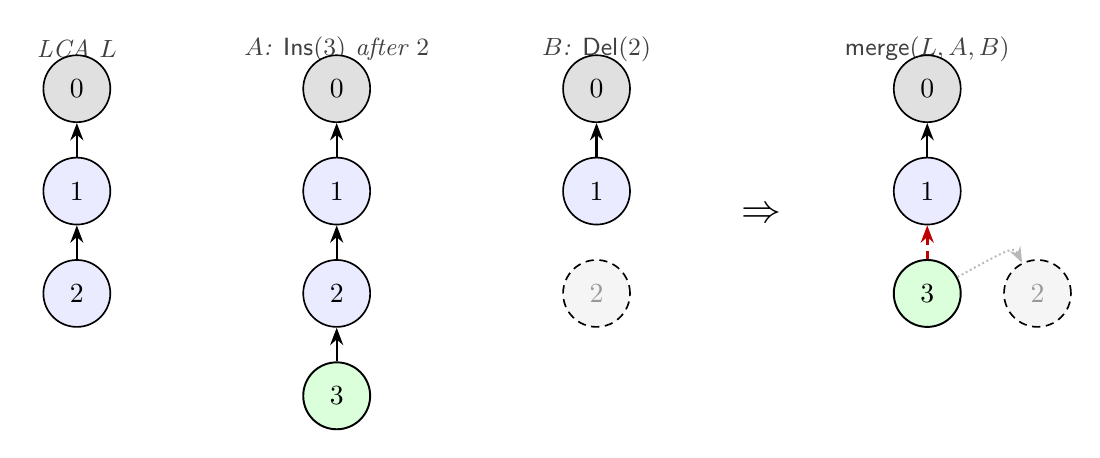
\begin{tikzpicture}
  % --- L ---
  \node[capt] at (0,0.5) {LCA $\lca$};
  \node[rootvtx] (lr) at (0,0)    {$0$};
  \node[vtx]     (l1) at (0,-1.3) {$1$};
  \node[vtx]     (l2) at (0,-2.6) {$2$};
  \draw[anc] (l1) -- (lr);
  \draw[anc] (l2) -- (l1);

  % --- A ---
  \node[capt] at (3.3,0.5) {$A$: $\Ins(3)$ after $2$};
  \node[rootvtx] (ar) at (3.3,0)    {$0$};
  \node[vtx]     (a1) at (3.3,-1.3) {$1$};
  \node[vtx]     (a2) at (3.3,-2.6) {$2$};
  \node[newv]    (a3) at (3.3,-3.9) {$3$};
  \draw[anc] (a1) -- (ar);
  \draw[anc] (a2) -- (a1);
  \draw[anc] (a3) -- (a2);

  % --- B ---
  \node[capt] at (6.6,0.5) {$B$: $\Del(2)$};
  \node[rootvtx] (br) at (6.6,0)    {$0$};
  \node[vtx]     (b1) at (6.6,-1.3) {$1$};
  \node[dead]    (b2) at (6.6,-2.6) {$2$};
  \draw[anc] (b1) -- (br);

  % --- merge ---
  \node at (8.7,-1.6) {\Large $\Rightarrow$};
  \node[capt] at (10.8,0.5) {$\mrg(\lca,A,B)$};
  \node[rootvtx] (mr) at (10.8,0)    {$0$};
  \node[vtx]     (m1) at (10.8,-1.3) {$1$};
  \node[dead]    (m2) at (12.2,-2.6) {$2$};
  \node[newv]    (m3) at (10.8,-2.6) {$3$};
  \draw[anc] (m1) -- (mr);
  \draw[climb] (m3) -- (m1);
  \node[ghost] (m3g) at (10.8,-2.6) {};
  \draw[ghost] (m3) .. controls (11.9,-2.0) .. (m2);
\end{tikzpicture}
\caption{Why merge converges. $3$ was born under $2$ (dotted, $2$'s ghost), but
$2$ is deleted on $B$. The merge climbs $3$'s birth-anchor up the \emph{LCA}
chain --- $2 \in \ids(\lca)\setminus I$, so $\climb_I(2)=\climb_I(\anc_\lca(2))=
\climb_I(1)=1$ --- and rehomes $3$ to $1$ (red dashed). The LCA is where ``$2$'s
parent is $1$'' is read. \textbf{No path on the operations is used.}}
\label{fig:merge}
\end{figure}

This is the whole reason a tombstone-free RGA can converge at all: the merge has
a third input, $\lca$, that retains the deleted node's ancestry. Keep that fact in
mind --- the next section is about the one place where there is \emph{no} such
third input.

\section{Why the path is necessary: a single replica has no LCA}
\label{sec:path}

Convergence of a replicated data type also requires that operations applied in
different orders on \emph{one} replica agree --- the framework discharges this as a
\emph{commutation} condition on $\doo$ (single-replica application). And here is
the catch: \textbf{$\doo$ has no LCA}. There is only the current state. So when an
insert's anchor has already been deleted, the parent the merge would have read
from $\lca$ is simply \emph{gone} --- unless the insert brought it along.

\paragraph{The counterexample (no path).} Take $\sigma=\{(1,A,0),(2,B,1)\}$ and the
two operations $\Ins(C, 2)$ (insert $C$ as id $3$ after $2$) and $\Del(2)$. Apply
them in both orders, with a \emph{prefix-free} insert (anchor only, no path):

\begin{figure}[h]
\centering
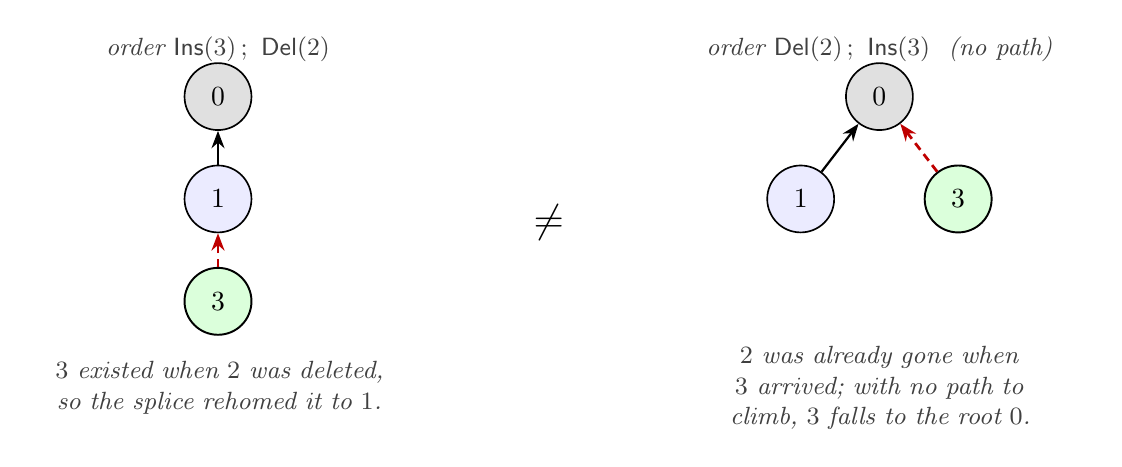
\begin{tikzpicture}
  % LEFT: Ins ; Del
  \node[capt] at (0,0.6) {order \(\Ins(3)\,;\ \Del(2)\)};
  \node[rootvtx] (lr) at (0,0)    {$0$};
  \node[vtx]     (l1) at (0,-1.3) {$1$};
  \node[newv]    (l3) at (0,-2.6) {$3$};
  \draw[anc] (l1) -- (lr);
  \draw[climb] (l3) -- (l1);
  \node[capt, text width=4.6cm, align=center] at (0,-3.7)
    {$3$ existed when $2$ was deleted, so the splice rehomed it to $1$.};

  % not equal
  \node at (4.2,-1.6) {\Large $\neq$};

  % RIGHT: Del ; Ins (no path)
  \node[capt] at (8.4,0.6) {order \(\Del(2)\,;\ \Ins(3)\) \ (no path)};
  \node[rootvtx] (rr) at (8.4,0)    {$0$};
  \node[vtx]     (r1) at (7.4,-1.3) {$1$};
  \node[newv]    (r3) at (9.4,-1.3) {$3$};
  \draw[anc] (r1) -- (rr);
  \draw[climb] (r3) -- (rr);
  \node[capt, text width=5.2cm, align=center] at (8.4,-3.7)
    {$2$ was already gone when $3$ arrived; with no path to climb, $3$ falls to
     the root $0$.};
\end{tikzpicture}
\caption{\textbf{Divergence without the path.} The same insert/delete pair, two
orders, two different trees: $3$ is anchored at $1$ on the left but at $0$ on the
right. The information ``$2$'s parent is $1$'' was destroyed by the tombstone-free
delete, and nothing on the right carries it. Mechanised as
\texttt{prefixfree\_diverges}.}
\label{fig:diverge}
\end{figure}

The two orders disagree on $3$'s anchor ($1$ versus $0$): the design does
\emph{not} commute. Because the delete physically removed $2$, the fact
``$\anc(2)=1$'' survives nowhere on the right --- and a prefix-free insert has no
way to reconstruct it.

\paragraph{The fix (carry the path).} Give the insert the ancestor path of its
anchor, $\Ins(C, [1], 2)$. Now when $2$ is dead, $\resolve$ climbs the carried
path $[1]$ to the live $1$, and both orders land $3$ under $1$ (Figure
\ref{fig:fix}). The path is exactly the ancestry that the tombstone-free state
threw away; carrying it on the operation restores commutation.

\begin{figure}[h]
\centering
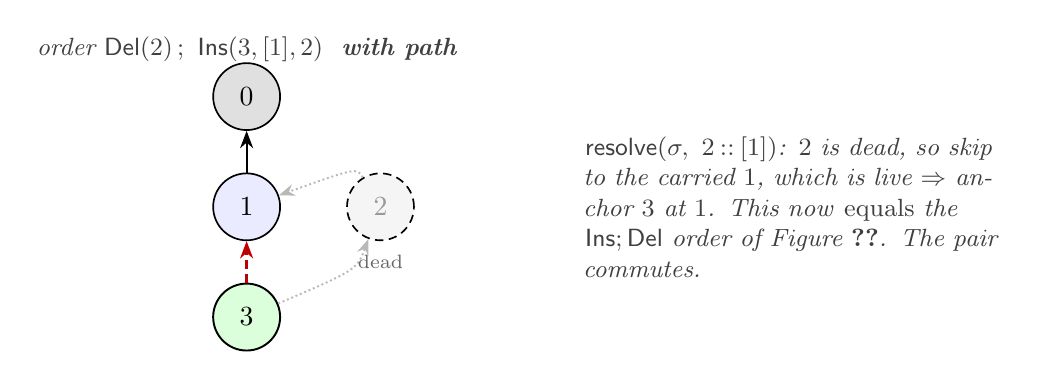
\begin{tikzpicture}
  \node[capt] at (0,0.6) {order \(\Del(2)\,;\ \Ins(3,[1],2)\) \ \textbf{with path}};
  \node[rootvtx] (rr) at (0,0)    {$0$};
  \node[vtx]     (r1) at (0,-1.4) {$1$};
  \node[dead]    (r2) at (1.7,-1.4) {$2$};
  \node[newv]    (r3) at (0,-2.8) {$3$};
  \draw[anc] (r1) -- (rr);
  \draw[climb] (r3) -- (r1);
  % climb illustration: 3 -> dead 2 -> 1
  \draw[ghost] (r3) .. controls (1.4,-2.2) .. (r2);
  \draw[ghost] (r2) .. controls (1.4,-0.9) .. (r1);
  \node[elbl, below=0.5mm of r2] {dead};
  \node[capt, text width=5.4cm, align=left] at (7.0,-1.4)
    {$\resolve(\sigma,\ 2\!::\![1])$: $2$ is dead, so skip to the carried $1$,
     which is live $\Rightarrow$ anchor $3$ at $1$. This now \emph{equals} the
     $\Ins;\Del$ order of Figure \ref{fig:diverge}. The pair commutes.};
\end{tikzpicture}
\caption{\textbf{The path restores convergence.} The carried path $[1]$ lets the
late insert climb past the deleted $2$ to the live $1$, matching the other order.
Mechanised as \texttt{prefix\_converges}.}
\label{fig:fix}
\end{figure}

\paragraph{The slogan.} \emph{A tombstone keeps the deleted node's parent in the
\textbf{state}; the path keeps it on the \textbf{operation}.} Remove the tombstone
and that parent has to ride along on any operation that might still need it --- and
on a single replica (no LCA) the insert is exactly such an operation. This is also
why the two are \emph{mutually exclusive but jointly unavoidable for the proof}: to
satisfy the $\doo$-commutation VC you may drop the tombstone or drop the path, but
not both. Dropping both defeats that route --- provably
(\texttt{RGA\_PrefixFree\_Impossible.lean}); the runnable witness that drops both
yet still converges \emph{via merge} is \texttt{RGA\_PrefixFree\_Impl.lean}.

\section{The path is ghost state: needed for the proof, not for execution}
\label{sec:ghost}

The previous section's ``necessary'' is a statement about the \emph{proof
obligation}, and its scope is worth being exact about: in a real execution the
path is \textbf{never read}. It is \emph{ghost state} --- pure proof scaffolding
that a runtime implementation can drop entirely.

Why it is never read comes down to how operations are generated. A client issues
an operation against \textbf{its own local replica}, on the state it currently
sees; you insert after, or delete, a node that is \emph{live in front of you}. On
any state where the anchor is live, \texttt{resolve} short-circuits on that anchor
and never inspects the prefix --- exactly what \texttt{ins\_path\_free} and
\texttt{del\_path\_free} prove. So for every operation a client can actually
\emph{issue}, the path is dead code. The one state that reads it --- an insert
whose anchor was \emph{already deleted on the same replica} --- is manufactured
only by the $\doo$-commutation VC, which quantifies over \emph{all} states and, in
forcing the two orders to agree, constructs exactly that intermediate. It sits
\textbf{outside the reachable set} (Figure~\ref{fig:ghost}).

\begin{figure}[h]
\centering
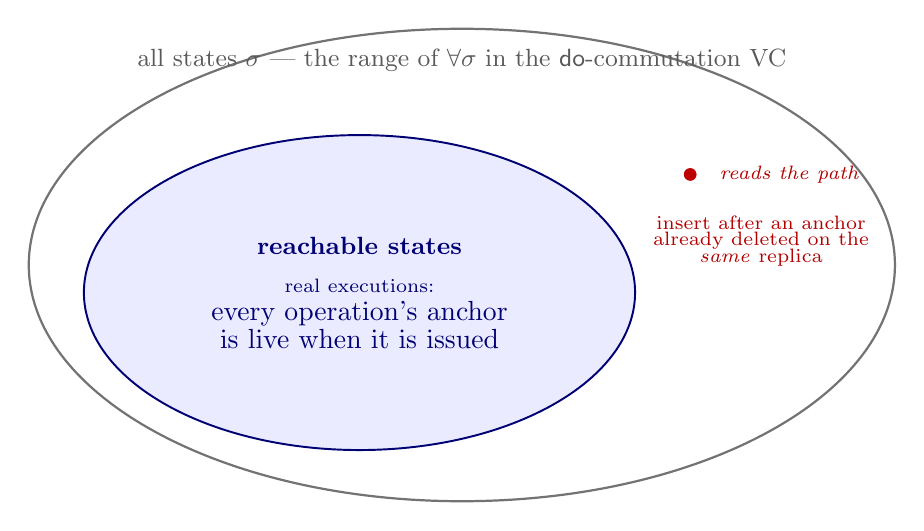
\begin{tikzpicture}
  \draw[line width=0.8pt, black!55] (0,0) ellipse (5.5 and 3.0);
  \node[black!65, font=\small] at (0,2.6)
    {all states $\sigma$ --- the range of $\forall\sigma$ in the $\doo$-commutation VC};
  \fill[blue!8] (-1.3,-0.35) ellipse (3.5 and 2.0);
  \draw[line width=0.7pt, blue!45!black] (-1.3,-0.35) ellipse (3.5 and 2.0);
  \node[blue!45!black, align=center] at (-1.3,-0.35)
    {\small\textbf{reachable states}\\[2pt]\scriptsize real executions:\\[-2pt]every operation's anchor\\[-2pt]is live when it is issued};
  \fill[red!75!black] (2.9,1.15) circle (2.3pt);
  \node[red!70!black, font=\scriptsize\itshape, anchor=west] at (3.15,1.15) {reads the path};
  \node[red!70!black, align=center, font=\scriptsize, anchor=north] at (3.8,0.75)
    {insert after an anchor\\[-2pt]already deleted on the\\[-2pt]\emph{same} replica};
\end{tikzpicture}
\caption{The path is ghost state. The $\doo$-commutation VC ranges over \emph{all}
states; real executions live in the shaded \emph{reachable} region, where every
operation's anchor is live and \texttt{resolve} short-circuits before the prefix
(\texttt{ins\_path\_free} / \texttt{del\_path\_free}). The path is consulted only at
the red state --- an insert whose anchor was already deleted on its own replica ---
which a voluntary, pull-based merge never produces.}
\label{fig:ghost}
\end{figure}

\paragraph{Why the system model rules it out.} Merge here is \textbf{voluntary},
pull-based --- like \texttt{git pull}. A replica's state does not change under its
feet: remote updates are incorporated only when the replica \emph{chooses} to
merge, at well-defined points, never in the middle of forming an operation. So the
anchor a client references is live when the operation is issued and stays live
until it is applied locally; the dead-anchor state never arises on the replica that
generated the op. And even in a model where remote state \emph{could} interleave,
the client can \textbf{reject an operation whose anchor is no longer present} --- a
cheap local check --- so the problematic state is never entered.

The upshot is a clean separation. The \emph{runtime} operations carry no path:
$\Ins$ needs only its immediate anchor, $\Del$ only its target, and the merge
recovers position from the LCA (\S\ref{sec:merge}). The path exists solely to
discharge the framework's universally-quantified commutation VC over states that no
execution produces. It is ghost state --- read by the proof, erased at run time.

\section{The asymmetry: $\Ins$ needs the path, $\Del$ does not}
\label{sec:asym}

Strikingly, only the \emph{insert} needs the path. A delete can always recompute
its target from the live state, because at the moment a delete runs, the node it
reparents \emph{to} (its target's parent) is still present. Figure
\ref{fig:asym} contrasts the two: the delete reads its answer from a node that is
alive \emph{now}; the insert may need a node that was alive \emph{then} but is
gone \emph{now}.

\begin{figure}[h]
\centering
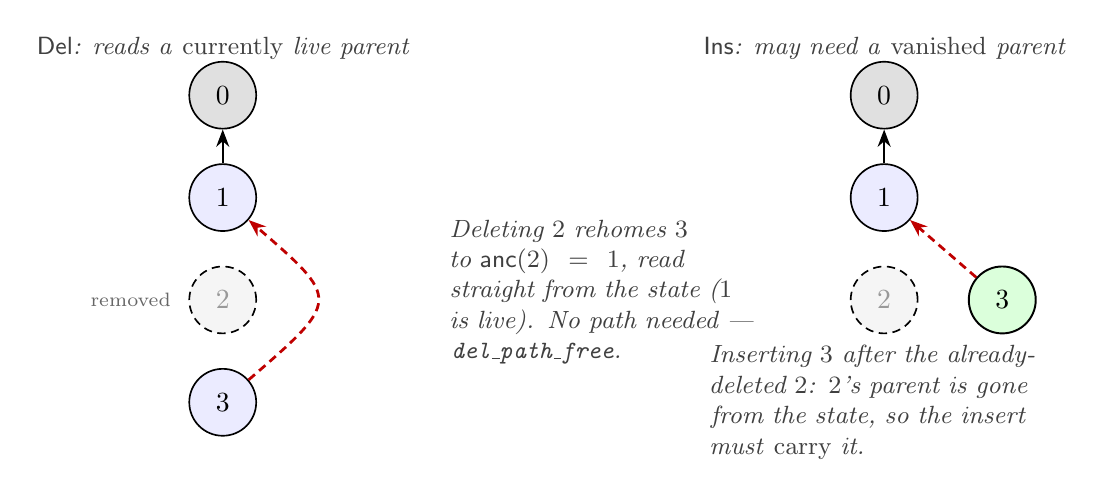
\begin{tikzpicture}
  % Del side
  \node[capt] at (0,0.6) {$\Del$: reads a \emph{currently} live parent};
  \node[rootvtx] (dr) at (0,0)    {$0$};
  \node[vtx]     (d1) at (0,-1.3) {$1$};
  \node[dead]    (d2) at (0,-2.6) {$2$};
  \node[vtx]     (d3) at (0,-3.9) {$3$};
  \draw[anc] (d1) -- (dr);
  \draw[climb] (d3) .. controls (1.5,-2.6) .. (d1);
  \node[elbl, left=1mm of d2] {removed};
  \node[capt, text width=4.0cm, align=left] at (4.9,-2.5)
    {Deleting $2$ rehomes $3$ to $\anc(2)=1$, read straight from the state ($1$ is
     live). No path needed --- \texttt{del\_path\_free}.};

  % Ins side
  \node[capt] at (8.4,0.6) {$\Ins$: may need a \emph{vanished} parent};
  \node[rootvtx] (ir) at (8.4,0)    {$0$};
  \node[vtx]     (i1) at (8.4,-1.3) {$1$};
  \node[dead]    (i2) at (8.4,-2.6) {$2$};
  \node[newv]    (i3) at (9.9,-2.6) {$3$};
  \draw[anc] (i1) -- (ir);
  \draw[climb] (i3) -- (i1);
  \node[capt, text width=4.4cm, align=left] at (8.4,-3.9)
    {Inserting $3$ after the already-deleted $2$: $2$'s parent is gone from the
     state, so the insert must \emph{carry} it.};
\end{tikzpicture}
\caption{The asymmetry. $\Del$ hands off children to a parent that is still live at
delete time, so it reads from state; a late $\Ins$ references a node that may have
been spliced away, so it must carry the path. (\texttt{del\_path\_free} /
\texttt{prefixfree\_diverges}.)}
\label{fig:asym}
\end{figure}

The intuition is temporal: a delete reparents \emph{all current children} the
instant it runs, keeping the forest connected; a concurrent (or reordered) insert
is a child that was \emph{not present} at that instant, so it missed the handoff
and must supply its own ancestry.

\section{Why no unconditioned proof exists}
\label{sec:uncond}

The path fixes the counterexample of \S\ref{sec:path}; it is natural to hope the
fixed design then discharges the standard framework schema as-is --- the flat
verification conditions, in which \emph{commutation is an equation over all
states}: for every concurrent pair left unordered by the reconciliation policy
$\rc$, $\doo(\doo(\sigma,a),b) = \doo(\doo(\sigma,b),a)$ for \emph{every}
$\sigma$, with the policy itself constrained (every non-commuting concurrent
pair must be $\rc$-oriented, and $\rc$-edges must not chain). That hope fails
twice, in instructive ways, and the failures are why this data type is verified
through the \emph{conditioned} framework instead.

\paragraph{Attempt 1: no path at all (the splice predecessor).} The original
tombstone-free design was the path-free splice RGA (\texttt{RGA\_Splice}, parked
on branch \texttt{wip/rga-splice}): an $\Ins$ carried only its immediate anchor,
a $\Del$ only its target, and delete physically spliced the node out. Physical
splice destroys the deleted node's parent pointer, so $\Ins$-after-$x$ and
$\Del(x)$ do not commute; whether the insert ran before the splice decides
whether it gets rehomed onto $\anc(x)$ or left dangling. The schema then
\emph{forces} an $\rc$-edge ordering the pair --- which makes the ordered-pair
commutation obligation (\texttt{cond\_comm\_base}) non-vacuous, and that
obligation is refuted by a three-operation trace
(Figure~\ref{fig:splice}).

\begin{figure}[h]
\centering
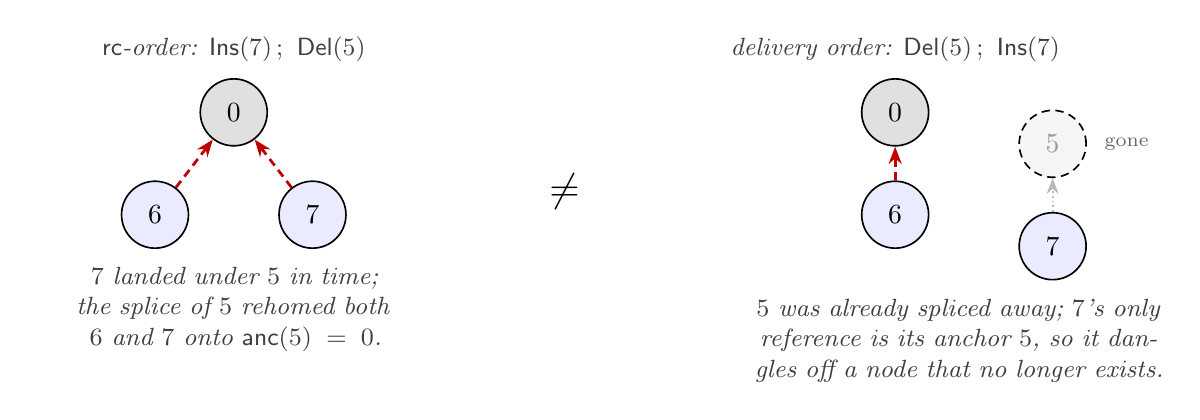
\begin{tikzpicture}
  % LEFT: rc order Ins ; Del
  \node[capt] at (0,0.8) {$\rc$-order: \(\Ins(7)\,;\ \Del(5)\)};
  \node[rootvtx] (lr) at (0,0)    {$0$};
  \node[vtx]     (l6) at (-1,-1.3) {$6$};
  \node[vtx]     (l7) at (1,-1.3)  {$7$};
  \draw[climb] (l6) -- (lr);
  \draw[climb] (l7) -- (lr);
  \node[capt, text width=5.0cm, align=center] at (0,-2.5)
    {$7$ landed under $5$ in time; the splice of $5$ rehomed both $6$ and $7$
     onto $\anc(5)=0$.};

  \node at (4.2,-1.0) {\Large $\neq$};

  % RIGHT: delivery order Del ; Ins
  \node[capt] at (8.4,0.8) {delivery order: \(\Del(5)\,;\ \Ins(7)\)};
  \node[rootvtx] (rr) at (8.4,0)    {$0$};
  \node[vtx]     (r6) at (8.4,-1.3) {$6$};
  \node[dead]    (r5) at (10.4,-0.4){$5$};
  \node[vtx]     (r7) at (10.4,-1.7){$7$};
  \draw[climb] (r6) -- (rr);
  \draw[ghost] (r7) -- (r5);
  \node[elbl, right=1mm of r5] {gone};
  \node[capt, text width=5.2cm, align=center] at (9.2,-2.9)
    {$5$ was already spliced away; $7$'s only reference is its anchor $5$, so it
     dangles off a node that no longer exists.};
\end{tikzpicture}
\caption{\textbf{The splice design fails the schema.} Start from root $0$, node
$5$ under $0$, node $6$ under $5$ (an earlier $\Ins$-after-$5$). The concurrent
pair $\Ins(7\ \text{after}\ 5) \parallel \Del(5)$ does not commute, so the
schema forces an $\rc$-edge (insert first). But replaying the mandated order
against the delivery order diverges at $7$: rehomed onto the root on the left,
dangling on the right. \texttt{cond\_comm\_base} is false for this design
(branch \texttt{wip/rga-splice}); no assignment of $\rc$ rescues it.}
\label{fig:splice}
\end{figure}

\paragraph{Attempt 2: the path --- which commutes only on truthful states.} The
path-carrying design of this note repairs the algebra, but look at the fine
print of the mechanised commutation fact (\texttt{rc\_non\_comm'}, \S\ref{sec:mech}):
it holds \emph{on accurate, fresh-id, root-not-stored states}. Those hypotheses
are not decoration. The unconditioned schema quantifies over \emph{all} states
and all operation payloads --- including operations whose recorded path
\emph{lies} --- and there the equation is false (Figure~\ref{fig:liar}): while
the anchor is alive the path is ignored (the insert reads the state), and once
the anchor is deleted the path is \emph{trusted} (the insert climbs the record);
if record and history disagree, the two orders read two different sources of
truth and diverge. No path discipline can be checked by $\doo$ locally ---
whether a path is accurate is a property of the \emph{execution} that produced
it, not of the state it is applied to.

\begin{figure}[h]
\centering
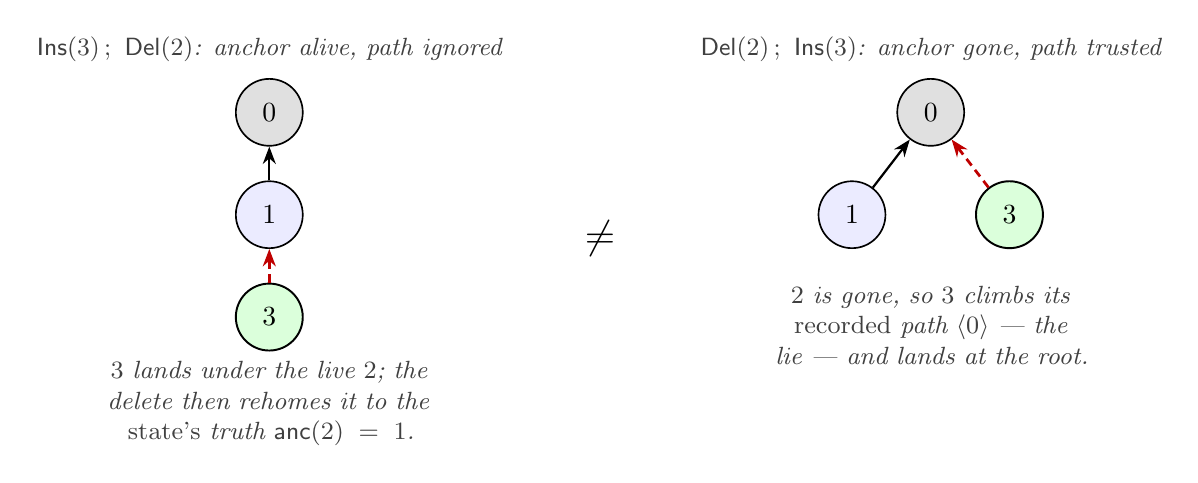
\begin{tikzpicture}
  % LEFT: Ins ; Del  (anchor alive, path ignored)
  \node[capt] at (0,0.8) {\(\Ins(3)\,;\ \Del(2)\): anchor alive, path ignored};
  \node[rootvtx] (lr) at (0,0)    {$0$};
  \node[vtx]     (l1) at (0,-1.3) {$1$};
  \node[newv]    (l3) at (0,-2.6) {$3$};
  \draw[anc] (l1) -- (lr);
  \draw[climb] (l3) -- (l1);
  \node[capt, text width=5.0cm, align=center] at (0,-3.7)
    {$3$ lands under the live $2$; the delete then rehomes it to the
     \emph{state's} truth $\anc(2)=1$.};

  \node at (4.2,-1.6) {\Large $\neq$};

  % RIGHT: Del ; Ins (anchor gone, lying path trusted)
  \node[capt] at (8.4,0.8) {\(\Del(2)\,;\ \Ins(3)\): anchor gone, path trusted};
  \node[rootvtx] (rr) at (8.4,0)    {$0$};
  \node[vtx]     (r1) at (7.4,-1.3) {$1$};
  \node[newv]    (r3) at (9.4,-1.3) {$3$};
  \draw[anc] (r1) -- (rr);
  \draw[climb] (r3) -- (rr);
  \node[capt, text width=5.4cm, align=center] at (8.4,-2.7)
    {$2$ is gone, so $3$ climbs its \emph{recorded} path $\langle 0\rangle$ ---
     the lie --- and lands at the root.};
\end{tikzpicture}
\caption{\textbf{A lying path breaks unconditioned commutation.} State: $1$
under $0$, $2$ under $1$. The operation $\Ins(3\ \text{after}\ 2)$ carries the
\emph{inaccurate} path $\langle 0 \rangle$ (claiming $2$ hangs off the root).
Left order: the path is never consulted and $3$ ends under $1$. Right order: the
path is consulted and $3$ ends under $0$. The schema's commutation equation
quantifies over such states and payloads, so it is unprovable; the mechanised
\texttt{rc\_non\_comm'} must and does assume accuracy.}
\label{fig:liar}
\end{figure}

\paragraph{Why this cannot be patched inside the schema.} Two escape routes
suggest themselves, and both are closed. \emph{Weakening the VC} --- baking
``accurate, fresh, root-free'' into the commutation statement --- silently
changes the schema: the framework's soundness theorem was proved for the
original VCs, so the modified bundle discharges nothing until that soundness
proof is redone (this project's costliest lesson; the redone proof \emph{is} the
conditioned framework). \emph{Re-engineering the operations} --- finding some
tombstone-free design whose operations commute unconditionally --- is refuted in
general: \texttt{RGA\_PrefixFree\_Impossible.lean} shows no tombstone-free,
prefix-free, local design can satisfy the $\rc=\Either$ commutation VC, and
ordering the insert/delete pair instead founders on rehoming non-transitivity
(\texttt{RGA\_DepComp\_Gate}).

\paragraph{The resolution.} The side conditions are promoted to first-class
citizens: an \emph{invariant} on states, an \emph{applicability} discipline on
operation generation (a well-behaved replica only issues an $\Ins$ whose
recorded path is its actual view --- which is all any honest replica can do),
and commutation proved \emph{conditioned} on both, propagated along
reachability under honest delivery. That is the conditioned MRDT framework
(\texttt{Sal/ConditionedMRDTs/}; companion note
\texttt{mrdt-metatheory.pdf}), and this data type is its founding instance:
the end-to-end theorem
(\texttt{rga\_tombstone\_free\_ra\_linearizable3\_eq}) is RA-linearizability up
to observational equivalence at every reachable configuration under honest
delivery. The price of leaving the unconditioned schema is real --- the
tombstoned RGA discharges the flat VCs in ${\sim}170$ lines, while this data
type's conditioned chain runs to ${\sim}10{,}000$ --- and, by the results
above, unavoidable.

\section{What is mechanised}
\label{sec:mech}

Every figure corresponds to a Lean fact in
\texttt{Sal/MRDTs/RGA\_Tombstone\_Free/}:
\begin{itemize}
  \item \texttt{prefix\_converges} / \texttt{prefixfree\_diverges} --- Figures
        \ref{fig:diverge}--\ref{fig:fix}: with the path the pair commutes; drop it
        and the same accurate pair diverges. The \emph{insert} path is necessary.
  \item \texttt{del\_path\_free} / \texttt{deldel\_pathfree\_converges} --- Figure
        \ref{fig:asym}: the \emph{delete} path is dispensable; a $\Del$ reads its
        reparent target $\anc(\sigma,x)$ from the live state.
  \item \texttt{rc\_non\_comm'} --- the full commutation VC: on accurate,
        fresh-id, root-not-stored states, \emph{every} operation pair commutes.
  \item \texttt{RGA\_PrefixFree\_Impossible.lean} --- a parameterised theorem: no
        tombstone-free, prefix-free, local design can satisfy the $\rc=\Either$
        commutation VC.
  \item Figure \ref{fig:splice} --- the splice predecessor's \texttt{do}-level
        non-commutation and refuted \texttt{cond\_comm\_base}: branch
        \texttt{wip/rga-splice}
        (\texttt{Sal/MRDTs/RGA\_Splice/RGA\_Splice\_MRDT.lean}). Figure
        \ref{fig:liar} is definitional (the climb trusts the record); its
        schema-level content is that \texttt{rc\_non\_comm'}'s accuracy
        hypothesis cannot be dropped, which is what forces the conditioned
        framework (\S\ref{sec:uncond}).
  \item \texttt{RGA\_PrefixFree\_Impl.lean} --- the runnable counterpart of
        Figures \ref{fig:merge} and \ref{fig:diverge}: its \emph{merge} converges
        the concurrent case (LCA), yet its single-replica $\doo$ diverges
        (\texttt{merge\_converges\_concurrent} vs.\
        \texttt{single\_replica\_do\_diverges}).
\end{itemize}

\paragraph{One honest caveat.} The merge's $\climb$ is bounded by a fuel equal to
the node id, so its convergence relies on \emph{id-monotone} anchors
($\anc(t) < t$). That holds under monotone timestamp allocation but is \emph{not}
guaranteed by the forest shape alone; a non-monotone state can make $\climb$ run
out of fuel under merge (\texttt{merge\_breaks\_wf} in
\texttt{RGA\_Reachability\_Invariant.lean}). So Figure \ref{fig:merge}'s
convergence is a theorem about reachable, monotone states --- the precise extra
condition the soundness argument must carry.

\end{document}
